\subsection{Logic.player-Quellpaket}
    \subsubsection{Player}
        \begin{table}[H]
            \caption{Klasse Player}
            \begin{tabular}{p{2.5cm}  p{9.5cm}} 
                \hline
                \textbf{Eigenschaft} & \textbf{Beschreibung}\\
                \hline
                Name & Player\\
                Ort & Quellpaket \textit{logic.player}\\
                \hline
                Zweck &
                Bietet eine abstrakte Oberklasse für die \textit{Detective}-Klasse und die \textit{MisterX}-Klasse
                und implementiert dabei alle grundlegenden Funktionen die benötigt werden um als
                Spieler am Spielgeschehen teilzunehmen. Darunter zählen Bewertungsfunktionen für die KI die für alle Spieler gleich sind
                oder auch die Ticketverwaltung sowie die Wegfindung.
                \\
                \hline
                Struktur &
                \begin{itemize}
                    \itemsep0em
                    \item Hält alle grundlegenden Informationen über einen Spieler wie die Tickets in dem \textit{ticket}-\textit{Array},
                        die aktuelle Station in der \textit{currentStation}-Variable als \textit{Station}-Instanz und ob der Spieler durch die KI oder 
                        durch einen menschlichen Spieler gesteuert wird in der \textit{ai}-Variable als \textit{boolean}
                    \item Die \textit{getShortestWay}-Methode bietet die Möglichkeit den kürzesten Weg durch das Netz zu finden und macht dabei
                            gebrauch von der \textit{StationDistance}-Klasse
                    \item Fordert die implementierung der \textit{play}-Methode.
                    Dadurch lässt sich die KI der Detektive und die von MisterX gleich behandeln.
                \end{itemize}
                \\
                \hline
            \end{tabular}
        \end{table}
        \begin{figure}[H]
            \centering
            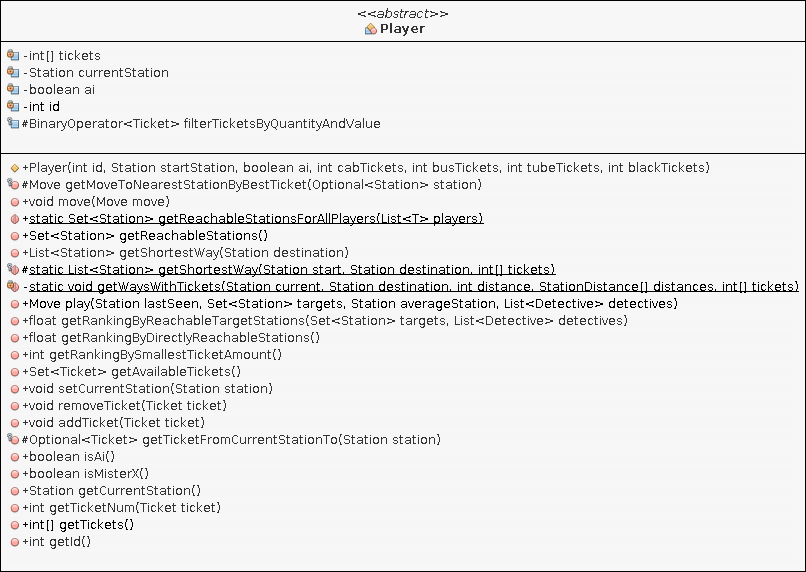
\includegraphics[scale=0.5]{img/uml/player.png}   
            \caption{Player UML-Klassendiagramm}
        \end{figure}


    \subsubsection{MisterX}
        \begin{table}[H]
            \caption{Klasse MisterX}
            \begin{tabular}{p{2.5cm}  p{9.5cm}} 
                \hline
                \textbf{Eigenschaft} & \textbf{Beschreibung}\\
                \hline
                Name & MisterX\\
                Ort & Quellpaket \textit{logic.player}\\
                \hline
                Zweck &
                Die \textit{MisterX}-Klasse erweitert die \textit{Player}-Klasse um Spezialisierungen um als Mister-X am Spielgeschehen teilzunehmen.
                Dazu gehören die Taktiken sowie die Bewertungsfunktionen und das Fahrtenbuch.
                \\
                \hline
                Struktur &
                \begin{itemize}
                    \itemsep0em
                    \item Hält in der \textit{logbook}-Variable das Fahrtenbuch welches als Liste von Tickets repräsentiert wird sowie 
                            die Station an der sich Mister-X zuletzt gezeigt hat in der \textit{lastSeen}-Variable als \textit{Station}-Instanz
                    \item Implementiert, wie von der Oberklasse vorgegeben, die \textit{play}-Methode
                    \item Macht beim vergleichen der Taktiken gebrauch von der \textit{TacticResult}-Klasse
                \end{itemize}\\
                \hline
            \end{tabular}
        \end{table}
        \begin{figure}[H]
            \centering
            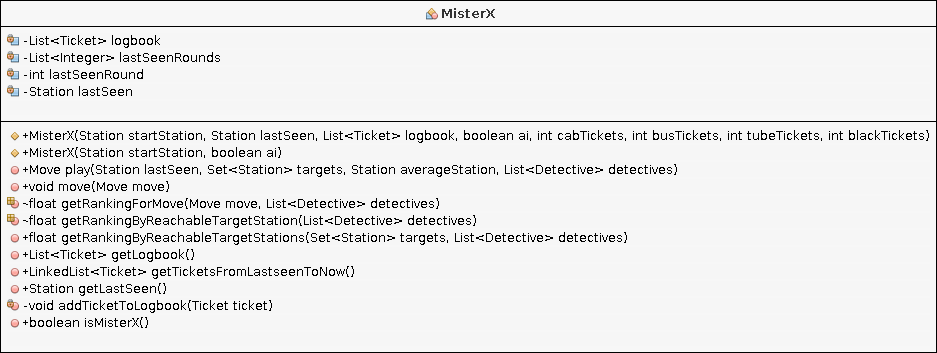
\includegraphics[scale=0.35]{img/uml/misterx.png}   
            \caption{MisterX UML-Klassendiagramm}
        \end{figure}



    \subsubsection{Detective}
        \begin{table}[H]
            \caption{Klasse Detective}
            \begin{tabular}{p{2.5cm}  p{9.5cm}} 
                \hline
                \textbf{Eigenschaft} & \textbf{Beschreibung}\\
                \hline
                Name & Detective\\
                Ort & Quellpaket \textit{logic.player}\\
                \hline
                Zweck &
                Die \textit{Detective}-Klasse erweitert die \textit{Player}-Klasse um Spezialisierungen um als Detektiv am Spielgeschehen teilzunehmen.
                Dazu gehören die Taktiken sowie die Bewertungsfunktionen
                \\
                \hline
                Struktur &
                \begin{itemize}
                    \itemsep0em
                    \item Implementiert, wie von der Oberklasse vorgegeben, die \textit{play}-Methode
                    \item Macht beim vergleichen der Taktiken gebrauch von der \textit{TacticResult}-Klasse
                \end{itemize}
                \\
                \hline
            \end{tabular}
        \end{table}
        \begin{figure}[H]
            \centering
            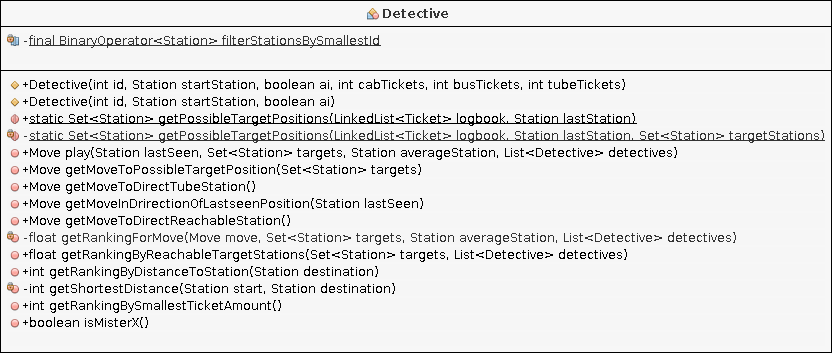
\includegraphics[scale=0.4]{img/uml/detective.png}   
            \caption{Detective UML-Klassendiagramm}
        \end{figure}


    \subsubsection{TacticResult}
        \begin{table}[H]
            \caption{Klasse TacticResult}
            \begin{tabular}{p{2.5cm}  p{9.5cm}} 
                \hline
                \textbf{Eigenschaft} & \textbf{Beschreibung}\\
                \hline
                Name & TacticResult\\
                Ort & Quellpaket \textit{logic.player}\\
                \hline
                Zweck &
                Die Hilfsklasse \textit{TacticResult} wird benötigt um die Taktiken miteinander zu vergleichen. 
                \\
                \hline
                Struktur &
                \begin{itemize}
                    \itemsep0em
                    \item Hält den Zug der Taktik als \textit{Move}-Instanz, die Identifikationsnummer und die Bewertung der Taktik.
                    \item Bietet einen Konstruktor der alle \textit{final} Attribute setzt
                    \item Bietet Getter-Methoden für die Attribute
                \end{itemize}
                \\
                \hline
            \end{tabular}
        \end{table}
        \begin{figure}[H]
            \centering
            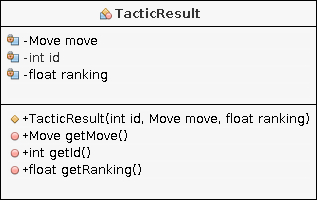
\includegraphics[scale=0.7]{img/uml/tacticResult.png}   
            \caption{TacticResult UML-Klassendiagramm}
        \end{figure}

    \subsubsection{StationDistance}
        \begin{table}[H]
            \caption{Klasse StationDistance}
            \begin{tabular}{p{2.5cm}  p{9.5cm}} 
                \hline
                \textbf{Eigenschaft} & \textbf{Beschreibung}\\
                \hline
                Name & StationDistance\\
                Ort & Quellpaket \textit{logic.player}\\
                \hline
                Zweck &
                Die Hilfsklasse \textit{StationDistance} wird für die Wegfindung benötigt und repräsentiert
                den Abstand von einer Station.
                Durch eine Menge von \textit{StationDistance} kann somit der kürzester Weg ermittelt werden. 
                \\
                \hline
                Struktur &
                \begin{itemize}
                    \itemsep0em
                    \item Hält eine \textit{Station}-Instanz welche die Station ist, die den Abstand hat der in der \textit{distance}-Variable gespeichert ist
                \end{itemize}
                \\
                \hline
            \end{tabular}
        \end{table}
        \begin{figure}[H]
            \centering
            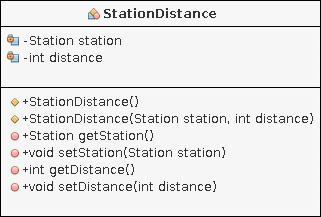
\includegraphics[scale=0.7]{img/uml/stationDistance.png}   
            \caption{StationDistance UML-Klassendiagramm}
        \end{figure}

